\documentclass{beamer}
\usepackage{amsmath}
\usepackage{xcolor}
\usepackage{multimedia}

\usetheme{copenhagen}
\definecolor{purple}{rgb}{0.3,0,0.4}
\definecolor{aqua}{rgb}{0,0.85,0.8}
\definecolor{grey}{rgb}{60,60,60}
\setbeamercolor*{palette primary}{use=structure, fg=white, bg=purple}
\setbeamercolor*{background canvas}{bg=purple!5}
\setbeamercolor*{block title example}{use=structure,fg=white,bg=purple}
\setbeamercolor*{block body example}{fg=black,use=block title,bg=purple!20}
\setbeamercolor*{block title}{use=example text,fg=white,bg=aqua!60!black}
\setbeamercolor*{block body}{fg=black,use=block title example,bg=aqua!10}

\usepackage{graphicx}
\usepackage{tikz-cd}
\usepackage{dsfont}
\usepackage[OT2,T1]{fontenc}
\usepackage{wrapfig}
\usepackage{multirow}
\DeclareSymbolFont{cyrletters}{OT2}{wncyr}{m}{n}
\DeclareMathSymbol{\Sha}{\mathalpha}{cyrletters}{"58}

\newcommand{\Gal}{\mathrm{Gal}}
\newcommand{\Cl}{\mathrm{Cl}}
\newcommand{\GL}{\mathrm{GL}}
\newcommand{\Ind}{\mathrm{Ind}}
\newcommand{\Reg}{\mathrm{Reg}}
\newcommand{\ord}{\mathrm{ord}}
\newcommand{\tors}{\mathrm{tors}}
\newcommand{\rk}{\mathrm{rk}}
\newcommand{\BSD}{\mathrm{BSD}}
\newcommand{\Tr}{\mathrm{Tr}}
\newcommand{\B}{\mathrm{B}}



\newcommand{\CC}{\mathbb{C}}
\newcommand{\FF}{\mathbb{F}}
\newcommand{\NN}{\mathbb{N}}
\newcommand{\PP}{\mathfrak{P}}
\newcommand{\QQ}{\mathbb{Q}}
\newcommand{\RR}{\mathbb{R}}
\newcommand{\ZZ}{\mathbb{Z}}
\newcommand{\GG}{\mathbb{G}}
\newcommand{\adele}{\mathbb{A}}
\newcommand{\pp}{\mathfrak{p}}
\newcommand{\qq}{\mathfrak{q}}
\newcommand{\rr}{\mathfrak{r}}
\newcommand{\af}{\mathfrak{a}}

\newcommand{\repnorm}[1]{\mathfrak{N}_{\QQ(#1) / \QQ}(#1)}

\theoremstyle{plain}
\newtheorem{thm}{Theorem}[section]
\newtheorem{rem}[thm]{Remark}
\newtheorem{proposition}[thm]{Proposition}
\newtheorem{conjecture}[thm]{Conjecture}
\newtheorem{deflem}[thm]{Definition/Lemma}
\newtheorem{question}[thm]{Question}



\graphicspath{ }


\title[Artin Formalism]{A Study of the Arithmetic Consequences of Artin Formalism for
Predicting Positive Rank}
\author{Edwina Aylward, Albert Lopez Bruch}
%\institute{LSGNT}
\date{21 May, 2024}

\begin{document}

\frame{\titlepage}

\begin{frame}
    \frametitle{Elliptic Curves}
    Let $K$ be a field. Any elliptic curve over $K$ can be written as the locus on $\mathbb{P}^2$ of a \textbf{Weierstrass equation}
    \begin{equation}
        E:y^2+a_1xy+a_3y=x^3+a_2x^2+a_4x+a_6,\quad a_i\in K
    \end{equation}
    together with $[0:1:0]$ at infinity, and it has an associated discriminant $\Delta\neq0$. 
    \\~\\
    When $\Delta=0$, the equation above defines a singular cubic curve, and two behaviours can occur.
    
    \centering
    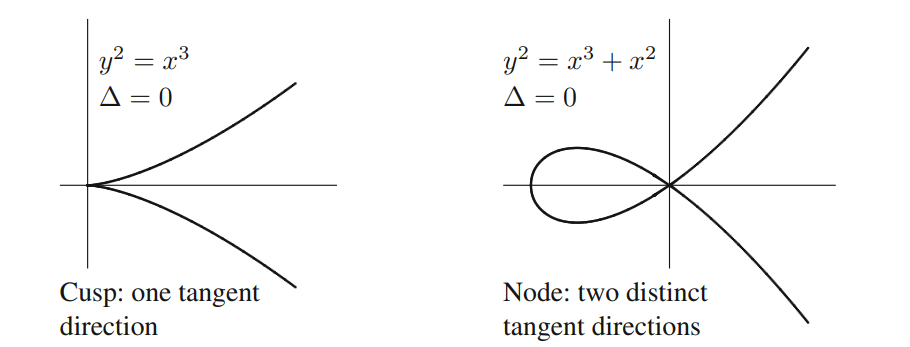
\includegraphics[scale=0.4]{Singular_cubic.png}
\end{frame}

\begin{frame}
    \frametitle{The Mordell-Weil Group}
    Let $K$ be a field and let $E$ be an elliptic curve over $K$. The set of $K$-points of $E$ form an abelian group $E(K)$. 
    \begin{theorem}[Mordell-Weil]
        Let $K$ be a number field and let $E$ be an elliptic curve over $K$. Then $E(K)$ is a finitely generated abelian group.
    \end{theorem}
    Consequently, $E(K)\cong E(K)_{tors}\times\ZZ^r$, where $r$ is denoted the \textbf{rank} of the elliptic curve.
    %\centering
    %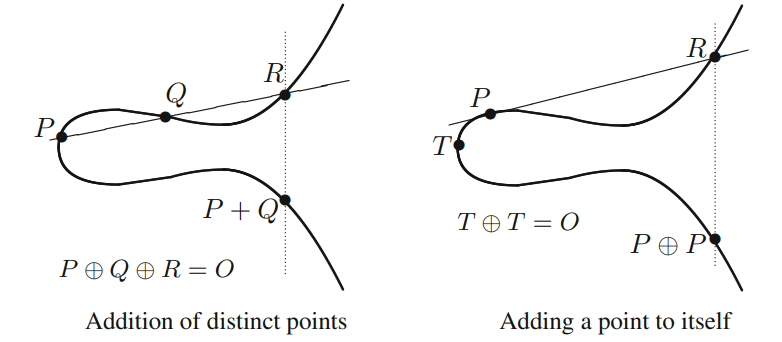
\includegraphics[scale=0.4]{MW_group.png}
\end{frame}

\begin{frame}
    \frametitle{Reduction of an Elliptic Curve}
    Suppose $K$ is a local field with $\mathrm{char}(K)=0$, discrete valuation $\nu$, valuation ring $R$ and max ideal $\mathfrak{m}$ and residue field $\kappa=R/\mathfrak{m}$.
    \begin{definition}
        A Weierstrass equation for $E/K$ is \textbf{minimal} if $a_i\in R$ and $\nu(\Delta)$ is minimal among all Weierstrass equations defining $E$.
    \end{definition}
    When the Weierstrass equation is minimal, we have an associated curve $\tilde{E}$ over $\kappa$ (which could be singular!) and a reduction map 
    $$\widetilde{(\cdot)}:E(K)\longrightarrow \tilde{E}(\kappa)$$
    by reducing the corrdinates modulo $\mathfrak{m}$.
\end{frame}

\begin{frame}
    \frametitle{Reduction Types}
    The reduction type of $E$ over $K$ describes the behaviour of $\tilde{E}/\kappa$.
    \begin{definition}
        We say that
        \begin{enumerate}%[label={(\alph*)}]
            \item $E/K$ has \textbf{good} reduction if $\tilde{E}$ is non-singular (i.e. $\nu(\Delta)=0$).
            \item $E/K$ has \textbf{multiplicative} reduction if $\tilde{E}$ has a node.
            \item $E/K$ has \textbf{additive} reduction if $\tilde{E}$ has a cusp.
        \end{enumerate}
        If $E/K$ has multiplicative reduction, then we say that the reduction is \textbf{split} if the slopes of the tangent lines at the node lie in $\kappa$, and \textbf{non-split} otherwise.
    \end{definition}

\end{frame}

\iffalse
\begin{frame}
    \frametitle{Reduction Types}
    The reduction type of $E$ over $K$ describes the behaviour of $\tilde{E}/\kappa$.
    \begin{definition}
        We say that
        \begin{enumerate}%[label={(\alph*)}]
            \item $E/K$ has \textbf{good} reduction if $\tilde{E}$ is non-singular (i.e. $\nu(\Delta)=0$).
            \item $E/K$ has \textbf{multiplicative} reduction if $\tilde{E}$ has a node.
            \item $E/K$ has \textbf{additive} reduction if $\tilde{E}$ has a cusp.
        \end{enumerate}
    \end{definition}
    \begin{proposition}
        Let $E$ be an elliptic curve over a local field $K$ of characteristic $0$. 
        \begin{enumerate}
            \item If $F/K$ unramified, the reduction of $E/K$ equals that of $E/F$.
            \item If $F/K$ is finite and $E/K$ is good or multiplicative, then $E/F$ has the same reduction.
            % \item If $E$ has non-split multiplicative reduction over $K$ and $F/K$ is a finite extension with even residual degree, then $E$ has split multiplicative reduction over $F$. 
            \item There exists a finite extension $F/K$ such that $E/F$ is either good or multiplicative.
        \end{enumerate}
    \end{proposition}
\end{frame}


\begin{frame}
    \frametitle{Multiplicative Reduction}
    \begin{definition}
        Suppose that $E/K$ has multiplicative reduction. Then we say that the reduction is \textbf{split} if the slopes of the tangent lines at the node lie in $\kappa$, and \textbf{non-split} otherwise.
    \end{definition}
    \begin{proposition}
        Let $E$ be an elliptic curve over a local field $K$ of characteristic $0$. 
        \begin{enumerate}
            \item If $F/K$ is finite and $E/K$ is split multiplicative, then $E/F$ has the same reduction.
            \item If $F/K$ has even residual degree and $E/K$ is non-split, then $E/F$ is split.
            \item There exists a finite extension $F/K$ such that $E/F$ is either good or split multiplicative.
        \end{enumerate}
    \end{proposition}   
\end{frame}
\fi



\begin{frame}
    \frametitle{L-function of an Elliptic Curve}
    Let $K$ be a number field and let $E$ be an elliptic curve over $K$.
    \begin{definition}
        If $\pp$ is a finite place of $K$, let $q_\pp=|\kappa_\pp|$ and $a_\pp=1+q_\pp-|\tilde{E}(\kappa_\pp)|$. The local polynomial of $E$ at $\pp$ is defined as
        \[
            P_\pp(E,T)=
            \begin{cases}
                1-a_\pp T+q_\pp T^2 &\text{ if $E/K_\pp$ good,}\\
                1-T &\text{ if $E/K_\pp$ split multiplicative,}\\
                1+T &\text{ if $E/K_\pp$ nonsplit multiplicative,}\\    
                1 &\text{ if $E/K_\pp$ additive.}
            \end{cases}
        \]
    Then the L-function attached to $E$ is 
    $$L(E/K,s)=\prod_{\pp\text{ prime}}\frac{1}{P_\pp(E,N(\pp)^{-s})}.$$
    \end{definition}
    We remark that $L(E/K,s)$ is holomorphic in some half plane.
\end{frame}

\begin{frame}
    \frametitle{Artin Representations}
    \begin{definition}
        Let $K$ be a field. An Artin representation $\rho$ is a complex finite dimensional vector space $V$ together with a homomorphism $\rho:G_K\to\GL(V)$ such that $\Gal(\bar{K}/F)\subseteq\ker\rho$ for some finite Galois extension $F/K$.
    \end{definition}
    Effectively, Artin representations of $K$ are finite dimensional reps of $\Gal(F/K)$ for some finite extension $F/K$.
    \begin{deflem}
        Let $L/K$ be a finite extension of number fields. If $\rho$ is an Artin representation of $L$, then the induction representation
        $$\Ind_{L/K}\rho:=\Ind_{G_L}^{G_K}\rho$$
        is an Artin representation of $K$.
    \end{deflem}
\end{frame}

\begin{frame}
    \frametitle{Artin Twists and Artin Formalism}
    Given an elliptic curve $E$ and an Artin representation $\rho$ over a number field $K$, we can construct an L-function $L(E/K,\rho,s)$.

    \begin{theorem}[Artin Formalism]
        Let $E$ be an elliptic curve over a number field $K$. 
        \begin{enumerate}
            \item For Artin representations $\rho_1,\rho_2$ over $K$,
            $$L(E/K,\rho_1\oplus\rho_2,s)=L(E/K,\rho_1,s)L(E/K,\rho_2,s).$$
            \item If $L/K$ is a finite extension and $\rho$ is an Artin representation over $L$,
            $$L(E/L,\rho,s)=L(E/K,\Ind_{L/K}\rho,s).$$
            \item If $L/K$ as above and 
            $\Ind_{L/K}\mathds{1}\cong\bigoplus_i\rho_i,$
            then 
            $$L(E/L,s)=\prod_i L(E/K,\rho_i,s).$$
        \end{enumerate}        
    \end{theorem}
\end{frame}

\begin{frame}
    \frametitle{An $S_3$ Example}
    Let $E$ be an elliptic curve over $\QQ$. Consider $L=\QQ(\sqrt[3]{2},\zeta_3)$ and note that $\Gal(L/\QQ)=S_3$. 
    \begin{table}[]
        \begin{tabular}{|c|c c c|}
            \hline
                        & $e$ & $(1,2)$ & $(1,2,3)$ \\ \hline
            $\mathds{1}$  & 1   & 1       & 1         \\ 
            $\varepsilon$ & 1   & -1      & 1         \\ 
            $\rho$        & 2   & 0       & -1        \\ \hline
        \end{tabular}
        \caption[short]{Character table for $S_3$}
    \end{table}
    By viewing all Artin reps as reps of $S_3$, Artin formalism gives
    \begin{itemize}
        \item $L(E/\QQ(\sqrt[3]{2},\zeta_3))=L(E,\mathds{1},s)L(E,\varepsilon,s)L(E,\rho,s)^2$
        \item $L(E/\QQ(\sqrt[3]{2}))=L(E,\mathds{1},s)L(E,\rho,s)$
        \item $L(E/\QQ(\zeta_3))=L(E,\mathds{1},s)L(E,\varepsilon,s)$.
    \end{itemize}
    Therefore,
    $$L(E/\QQ(\sqrt[3]{2},\zeta_3),s)L(E/\QQ,s)^2=L(E/\QQ(\zeta_3),s)L(E/\QQ(\sqrt[3]{2}),s)^2$$    
\end{frame}

\begin{frame}
    \frametitle{Birch and Swinnerton-Dyer Conjecture}
    \begin{conjecture}[Birch--Swinnerton-Dyer]
        Let $E$ be an elliptic curve defined over a number field $F$. Then 
        \begin{enumerate}%[label={\bfseries  BSD\arabic*.}]
            \item The rank of the Mordell-Weil group of $E$ over $F$ equals the order of vanishing of the $L$-function; that is,
            $$\ord_{s=1}L(E/F,s)=\rk E/F = r.$$
            \item The group $\Sha_{E / F}$ has finite order and the leading term of the Taylor series at $s=1$ of the $L$-function is
            \begin{equation*}\label{BSD_2}
                \lim_{s\to1}\frac{L(E/F,s)}{(s-1)^r}\cdot\frac{\sqrt{|\Delta_F|}}{\Omega_+(E)^{r_1+r_2}|\Omega_-(E)|^{r_2}}=\frac{\Reg_{E/F}|\Sha_{E/F}|C_{E/F}}{|E(F)_{\tors}|^2}.
            \end{equation*}
        \end{enumerate}
    \end{conjecture}
    

\end{frame}

\begin{frame}
    \frametitle{Birch and Swinnerton-Dyer for Artin Twists}
    \begin{definition}
        For an elliptic curve $E$ over a number field $K$, let
        $$\BSD(E/K):=\frac{\Reg_{E/K}|\Sha_{E/K}|C_{E/K}}{|E(K)_{\tors}|^2}.$$
    \end{definition}
    \begin{conjecture}[BSD1 for Artin Twists]
        Let $E/\QQ$ be an elliptic curve, $\rho$ an Artin representation and $F/\QQ$ a Galois extension $\QQ$ such that $\rho$ factors through $Gal(F/\QQ)$. Then
        $$\ord_{s=1}L(E,\rho,s)=\langle\rho,E(F)_\CC\rangle,$$
        where $E(F)_\CC=E(F)\otimes_\ZZ \CC$ is viewed as a $\Gal(F/\QQ)$ representation and $\langle\cdot,\cdot\rangle$ is the usual inner product of characters.
    \end{conjecture}
    \textbf{Problem:} Can we formulate a BSD2 analogue for Artin Twists?
\end{frame}

\begin{frame}
    \frametitle{Arithmetic and Analytic Information}
    The BSD conjecture gives a way to obtain arithmetic information from analytic and viceversa.
    \begin{example}
        Isogenous elliptic curves have the same L-function. Hence, BSD predicts that their rank and $\BSD$ terms with the periods are equal. The former is elementary, but the later is a deep result by Cassels.
    \end{example}
    \begin{example}
        Let $\rho$ be an Artin representation over $\QQ$ that factors through $\Gal(F/\QQ)$. If $\rho^\mathfrak{g}$ is the representation such that $\Tr\circ \rho^\mathfrak{g}=\mathfrak{g}(\Tr\circ\rho)$ for some $\mathfrak{g}\in\Gal(\QQ(\rho)/\QQ)$, then $$\langle\rho,E(F)_\CC\rangle=\langle\rho^\mathfrak{g},E(F)_\CC\rangle.$$
        One then expects that $\ord_{s=1}L(E,\rho,s)=\ord_{s=1}L(E,\rho^\mathfrak{g},s)$, but this is still a conjecture.
    \end{example}
\end{frame}

\begin{frame}
    \frametitle{Arithmetic and Analytic Information}
    \begin{example}
        From the $S_3$ example, BSD1 predicts that $$\rk E/\QQ(\sqrt[3]{2},\zeta_3)+2\rk E/\QQ=\rk E/\QQ(\zeta_3)+2\rk E/\QQ(\sqrt[3]{2}).$$
        Let $V=E(\QQ(\sqrt[3]{2},\zeta_3))\otimes_\ZZ \CC$, which is naturally a $\CC S_3$-module. Then
        \begin{itemize}
            \item $\rk E/\QQ=\dim V^{S_3}= \langle V,\mathds{1}\rangle$,
            \item $\rk E/\QQ(\zeta_3)=\dim V^{C_3}=\langle V,\mathds{1}\oplus\varepsilon\rangle$,
            \item $\rk E/\QQ(\sqrt[3]{2})=\dim V^{C_2}=\langle V,\mathds{1}\oplus\rho\rangle$,
            \item $\rk E/\QQ(\sqrt[3]{2},\zeta_3)=\dim V=\langle V,\mathds{1}\oplus\varepsilon\oplus\rho^2\rangle$.
        \end{itemize}
    \end{example}

\end{frame}

\begin{frame}
    
\end{frame}

\begin{frame}
    \frametitle{Local Data: Tamagawa Numbers}
    We now begin our study of the $C_{E/K}$ factor, upon which the test depends. 

    \begin{definition}[Tamagawa Numbers]
        Let $E$ be an elliptic curve over a local field $K$ and let $\tilde{E}_{ns}(\kappa)\subseteq \tilde{E}(\kappa)$ be the non-singular points of the reduction curve. Then $E_0(K):=\{P\in E(K):\tilde{P}\in \tilde{E}_{ns}(\kappa)\}$ is a subgroup of $E(K)$ and the \textbf{Tamagawa Number} of $E/K$ is defined as $$c(E/K)=[E(K):E_{0}(K)].$$
        Naturally, if $K$ is a number field and $\pp$ is a finite place, then
        $$c_\pp(E/K):=c(E/K_\pp).$$
    \end{definition}
    It is clear from the definition that if $E/K$ has good reduction, then $c(E/K)=1$.
\end{frame}

\begin{frame}
    \frametitle{Tamagawa Numbers of Multiplicative Reduction}
    Tamawaga numbers can always be computed using Tate's algorithm. When $E/K$ is multiplicative, then Tamagawa numbers have a simple description.
    \begin{lemma}
        Suppose that $E/K$ has multiplicative reduction and let $n=\nu(\Delta^{\min})$. Then
        \[
        c(E/K)=
        \begin{cases}
            n\quad \text{ if $E/K$ is split,}\\
            1\quad \text{ if $n$ is odd and $E/K$ is non-split,}\\
            2\quad \text{ if $n$ is even and $E/K$ is non-split,}
        \end{cases}    
        \] 
    \end{lemma}

    For addtive reduction there is also an explicit description as long as $\mathrm{char}(\kappa)\neq 2,3$, but the expressions are more involved.

\end{frame}

\begin{frame}
    \frametitle{The Semistable Reduction Theorem}
    To study Tamagawa numbers in our context, we need to understand how reduction types change under finite extensions.
    \begin{lemma}
        Let $E$ be an elliptic curve over a local field $K$ of characteristic $0$ and let $F/K$ be a finite extension.
        \begin{enumerate}
            \item If $F/K$ unramified, the reduction of $E/K$ equals that of $E/F$.
            \item If $E/K$ is good or multiplicative, then $E/F$ has the same reduction.
            \item If $E/K$ is non-split multiplicative, then $E/F$ is split multiplicative if and only if $F/K$ has even residual degree. 
            \item There exists a finite extension $L/K$ such that $E/L$ is either good or split multiplicative.
        \end{enumerate}
    \end{lemma}    

\end{frame}

\begin{frame}
    \frametitle{Local Data: The Minimal Discriminant}
    Apart from the Tamagawa numbers, a second local term appears in the $C_{E/K}$ term arising from the minimal discriminant.
    \begin{definition}
        Let $E/\QQ$ be an elliptic curve and let $\Delta$ a \textbf{global minimal differential}. Let $K$ be a number field and $\pp$ a prime of $K$. If $\Delta_{\pp}^{\min}$ is the minimal differential of $E/K_\pp$, then we define 
        $$d_\pp(E/K)=\left|\frac{\Delta_\pp^{\min}}{\Delta}\right|^{1/12}.$$
    \end{definition}
\end{frame}

\begin{frame}
    \frametitle{Properties of the $d_\pp$ Terms}
    Similarly to Tamagawa numbers, we need to understand important properties of the terms $d_\pp(E/K)$.
    \begin{lemma}
        Let $K$ be a number field and let $\pp$ be a prime of $K$ above $p$. If $p$ is unramified in $K/\QQ$ or $E/\QQ_p$ is good or multiplicative, then $\Delta_\pp^{\min}=\Delta$ and so $d_\pp(E/K)=1$.
    \end{lemma}
    
    Thus, $d_\pp(E/K)>1$ only if $p$ ramifies in $K/\QQ$ and $E/\QQ_p$ is additive. If $p\neq 2,3$ there are also explicit descriptions for these terms.

\end{frame}

\begin{frame}
    \frametitle{Example (maybe dihedral --> The unit example from Vladimir)}
        
\end{frame}



\begin{frame}
    
\end{frame}


\begin{frame}
    \frametitle{Consistency with the Cyclic Case}
    We have now seen some examples where the Norm Relations test predicts positive rank. When the extension is cyclic, however, the test will never predict rank growth.

    \begin{lemma}
        Let $\rho$ be a representation of the cyclic group $C_d$. Then there is one unique relation $\Theta_\rho\in \B(C_d)$ such that 
        $$\CC[C_d/\Theta_{\rho}]=\repnorm{\rho}=\bigoplus_{\mathfrak{g}\in\Gal(\QQ(\rho)/\QQ)}\rho^{\mathfrak{g}}.$$
        In particular, if $\rho=\psi_d$ is a faithful character of $C_d$, then
        $$\Theta_{\psi_d}=\sum_{k\mid d}\mu(k)C_k.$$
    \end{lemma}

\end{frame}

\begin{frame}
    \frametitle{$C_{12}$ Example}
    Let $F/K$ be a Galois extension with $\Gal(F/K)=C_{12}$ and let $\psi$ be a faithful character.

    \begin{figure}[!ht]
        \centering
        \begin{tikzpicture}

            \node (Q1) at (-3,0) {$K$};
            \node (Q2) at (-4,1) {$L_3$};
            \node [red] (Q3) at (-1,2) {$L_4$};
            \node [red] (Q4) at (-2,1) {$L_2$};
            \node [red] (Q5) at (-2,3) {$F$};
            \node [red] (Q6) at (-3,2) {$L_6$};

            \node (Q7) at (1,0) {$C_{12}$};
            \node (Q8) at (0,1) {$C_4$};
            \node [red] (Q9) at (3,2) {$C_3$};
            \node [red] (Q10) at (2,1) {$C_6$};
            \node [red] (Q11) at (2,3) {$C_1$};
            \node [red] (Q12) at (1,2) {$C_2$};
            

            \draw (Q1)--(Q2) node [pos=0.8, below,inner sep=0.4cm] {};
            \draw (Q1)--(Q4) node [pos=0.8, below,inner sep=0.4cm] {};
            \draw (Q2)--(Q6) node [pos=0.8, below,inner sep=0.4cm] {};
            \draw [red] (Q3)--(Q5) node [pos=0.8, below,inner sep=0.4cm] {};
            \draw [red] (Q4)--(Q6) node [pos=0.8, below,inner sep=0.4cm] {};
            \draw [red] (Q6)--(Q5) node [pos=0.8, below,inner sep=0.4cm] {};
            \draw [red] (Q4)--(Q3) node [pos=0.8, below,inner sep=0.4cm] {};

            \draw (Q7)--(Q8) node [pos=0.8, below,inner sep=0.4cm] {};
            \draw (Q7)--(Q10) node [pos=0.8, below,inner sep=0.4cm] {};
            \draw (Q8)--(Q12) node [pos=0.8, below,inner sep=0.4cm] {};
            \draw [red] (Q9)--(Q11) node [pos=0.8, below,inner sep=0.4cm] {};
            \draw [red] (Q10)--(Q12) node [pos=0.8, below,inner sep=0.4cm] {};
            \draw [red] (Q12)--(Q11) node [pos=0.8, below,inner sep=0.4cm] {};
            \draw [red] (Q10)--(Q9) node [pos=0.8, below,inner sep=0.4cm] {};
        \end{tikzpicture}
    \end{figure}
    \begin{align*}
        \Ind_{C_1}^{C_{12}}\mathds{1}=\oplus_{a=0}^{11}\psi^a,&\quad\quad\Ind_{C_2}^{C_{12}}\mathds{1}=\oplus_{a=0}^{5}\psi^{2a},\\
        \Ind_{C_4}^{C_{12}}\mathds{1}=\oplus_{a=0}^{3}\psi^{3a},&\quad\quad\Ind_{C_6}^{C_{12}}\mathds{1}=\oplus_{a=0}^{1}\psi^{6a},\\
        \Ind_{C_1}^{C_{12}}\mathds{1}\ominus\Ind_{C_2}^{C_{12}}\mathds{1}\ominus\Ind&_{C_3}^{C_{12}}\mathds{1}\oplus\Ind_{C_6}^{C_{12}}\mathds{1}=\bigoplus_{(a,12)=1}\psi^a
    \end{align*}
\end{frame}

\begin{frame}
    \frametitle{Consistency with the Cyclic Case}
    The main result is the following.
    \begin{thm}\label{thm_consistent_cyclic}
        Let $d\geq2$ be a positive integer and let $F/K$ be a Galois extension of number fields such that $\Gal(F/K)=C_d$. Let $\rho$ be a representation of $C_d$ and let $\Theta_\rho\in \B(C_d)$ be such that
        $$\CC[G/\Theta_\rho]=\repnorm{\rho}.$$
    
        If $E/\QQ$ is a semistable elliptic curve at $2$ and $3$, then for any $\QQ(\sqrt{D})\subseteq\QQ(\rho)$,
        $$C(\Theta_\rho)\in N_{\QQ(\sqrt{D})/\QQ}(\QQ(\sqrt{D})^{\times}).$$
    \end{thm}

\end{frame}


\begin{frame}
    \frametitle{Simplification to Faithful Characters}

    \begin{lemma}
        Suppose that the Theorem holds for faithful characters $\psi_d$ of $C_d$. Then it also holds for any representation $\rho$ of $C_d$.
    \end{lemma}

    Ideas for the proof:
    \begin{enumerate}
        \item If $\psi_{d'}$ is another character of order $d'$, then we can view it as a faithful character of $C_{d'}=\Gal(F/F^{C_{d'}})$.
        \item For any representation $\rho$ of $C_d$, $\repnorm{\rho}$ is a rational representation.
        \item The basis for the rational representations of $C_d$ is 
        $$\left\{\chi_k:=\repnorm{\psi_k}:k\mid d\right\},$$
        where $\psi_k$ is a character of order $k$.
    \end{enumerate}

\end{frame}

\begin{frame}
    \frametitle{Strategy for the Proof of the Theorem}
    The outline for the proof is the following.
    \begin{enumerate}
        \item Proof for $\Gal(F/K)=C_{q}$ where $q$ is an odd prime.
        \item Proof for $\Gal(F/K)=C_{qr}$ where $q,r$ are distinct odd primes.
        \item An inductive reasoning gives the proof for $\Gal(F/K)=C_d$ is an odd extension.
        \\~\\
        However, when $d$ is even more care is required.
        \item Prove separately the cases $\Gal(F/K)=C_4, C_{2q}, C_{4q}, C_{8q}$ where $q$ is an odd prime.
        \item A similar inductive reasoning gives the proof for $d$ even.
    \end{enumerate}
    
    Furthermore, to prove each case, we fix some prime $\pp$ of $K$ and study the `local contribution' $C_\pp(\Theta_d)$ of the primes above $\pp$ is the corresponding fields.
\end{frame}

\begin{frame}
    \frametitle{Quadratic Subfields of Cyclotomic Extensions}
    If $\psi_d$ is a faithful character of $C_d$, then $\QQ(\psi_d)=\QQ(\zeta_d)$ where $\zeta_d$ is a primitive $d$-th root of unity.

    \begin{lemma}
        Let $p$ be an odd prime and let $p^*=(-1)^{(p-1)/2}p$. Then
        \begin{itemize}
            \item $\QQ(\sqrt{p^*})$ is the unique quadratic subfield of $\QQ(\zeta_{p})$.
            \item $\QQ(i), \QQ(\sqrt{\pm p})$ are the unique quadratic subfields of $\QQ(\zeta_{4p})$.
        \end{itemize}
    \end{lemma}
    \begin{proof}
        The number of quadratic subfields is determined by Galois correspondence. Also, $p$ is the only prime that ramifies in $\QQ(\zeta_p)$, and the only quadratic subfield unramified outside $p$ is $\QQ(\sqrt{p^*})$. The second part is similar with ramification at $2$ and $p$.
    \end{proof}
\end{frame}


\begin{frame}
    \frametitle{The $C_q$ Case: Multiplicative Reduction}
    If $\Gal(F/K)=C_q$ then $\Theta_q=C_1-C_q$. Let $\pp$ be a prime of $K$ such that $E/K_\pp$ has multiplicative reduction.

    \begin{table}[!ht]
        \centering
        \begin{tabular}{|l|l|l|l|l|}
        \hline
        $e_\pp$ & $f_\pp$  & $c(E/K_\pp)$ & $\prod_{\PP\mid\pp}c(E/F_\PP)$  & $C_\pp(\Theta_q)$ \\ \hline
        $1$ & $1$ & $n;\tilde{n}$ & $n^q;\tilde{n}^q$ & $\square$ \\ \hline
        $q$ & $1$ & $n;\tilde{n}$ & $qn;\tilde{n}$ & $q\square;\square$ \\ \hline
        $1$ & $q$ & $n;\tilde{n}$ & $n;\tilde{n}$ & $\square$ \\ \hline
        \end{tabular}
    \end{table}
    From this it is clear we need to show that 

    \begin{lemma}[1]
        Let $q$ be an odd prime. Then $q$ is a norm from $\QQ(\sqrt{q^*})$.
    \end{lemma}
    
    
    

\end{frame}
    

\begin{frame}
    \frametitle{The $C_q$ Case: Additive Reduction}
    If $E/K_\pp$ is additive and $\PP\mid\pp$ is a prime in $F$ above $\pp$, then the minimal discriminants agree unless $\pp$ is totally ramified in $F/K$. In that case, $d_\PP(E/F)$ is a power of $N(\pp)$. So we need to show the following.
    \begin{lemma}[2]
        Let $\pp$ be a prime on a number field $K$ that ramifies in a $C_q$ extension of $K$. Then $N(\pp)$ is a norm from $\QQ(\sqrt{q^*})$.
    \end{lemma}
    

\end{frame}


\begin{frame}
    \frametitle{Proof of Lemma 1}
    \begin{lemma}
        Let $q\equiv1\pmod{4}$. Then the fundamental unit of $\QQ(\sqrt{q})$ is negative.
    \end{lemma}
    \begin{proof}[Proof of Lemma 1]
        If $q\equiv 3\pmod{4}$, then $N(\sqrt{q^*})=N(\sqrt{-q})=q$. If $q\equiv 1\pmod{4}$ and $\epsilon$ is a fundamental unit, then $N(\epsilon\sqrt{q})=N(\epsilon)N(\sqrt{q})=(-1)(-q)=q$. 
    \end{proof}
\end{frame}


\begin{frame}
    \frametitle{Proof of Lemma 2}
    
\end{frame}






\begin{frame}
    \frametitle{End}

    

\end{frame}

\end{document}